\title{Expectation Maximization}
\label{chp:label}
\author{Bruno Almeida Pimentel}
\institute{Instituto de Computação - Universidade Federal de Alagoas}
\maketitle


%\chapter{Optimization}

Expectation Maximization (EM) is one of the most frequently used algorithms for clustering in Machine Learning \cite{moon1996expectation, do2008expectation}. Its popularity comes from the underlying simplicity of the algorithm. EM can be used in a number of applications, such as Data Mining, Clustering, Natural Language Processing, Signal Processing, Medical Image Reconstruction amongst others \cite{dellaert2002expectation, dempster1977maximum, ceppellini1955estimation, tzoreff2017expectation, li2019expectation}. This chapter is aimed at providing the reader with knowledge for understanding and using the EM method. Furthermore, readers can exercise their knowledge by implementing the method based on the provided definitions. 

%This chapter is organized as follows. Section \ref{sec:coin} shows an experiment with a coin-flipping in order to explain the mathematical intuition behind the EM algorithm. Section \ref{sec:math} presents the mathematical foundations of EM. Section \ref{sec:algorithm} introduces the EM algorithm. And Section \ref{sec:applications} depicts some cases of real world applications of the EM algorithm. 


\section{Intuition Behind the EM clustering algorithm}

This section is aimed at providing the reader with the basic underlying idea of the EM method operation. Two practical experiments are discussed in order to expose the main steps of the method.

\subsection{A coin-flipping experiment}
\label{sec:coin}

With the aim of explaining the mathematical intuition as well as the Expectation Maximization algorithm operation, this section focuses on a simple coin-flipping experiment. So, suppose that we want to estimate the bias of two coins. Also, consider that these coins can be fair or not (i.e., they can be more heavily weighted on their heads face, for example). This experiment is based on steps where each one consists of two main actions:

\begin{itemize}
    \item Randomly choose a coin;
    \item Flip the chosen coin $10$ times.
\end{itemize}

After carrying out these steps $6$ times, we may achieve the result presented in the table below (where H means heads and T means tails):

\begin{center}
\begin{tabular}{|c|c|c|c|c|} 
 \hline
 \textbf{Steps} &\textbf{Coin} & \textbf{Trial} & \textbf{\# coin A heads} & \textbf{\# coin B heads} \\ \hline 
1 & A & HTTTHHTHTH & 5 & 0\\ \hline 
2 & B & HHHHTHHHHH & 0 & 9\\ \hline
3 & B & HTHHHHHTHH	& 0 & 8\\ \hline 
4 & B & HTHTTTHHTT & 0 & 4\\ \hline
5 & A & THHHTHHHTH & 7 & 0\\ \hline 
6 & B & HTTHTHHHHH & 0 & 7\\ \hline
\end{tabular}
\end{center}

To independently estimate each coin's bias, we must consider the total of heads and the total of flips. For coin A, the total of flips is $20$ ($2$ flips trials of $10$ flips each one). Thus, the bias of coin A would be 12/20. Similarly, for coin B the bias is 28/40. Therefore, when we know which coin was flipped, the problem of estimating the coin's bias can be solved as above. However, what about if we do not know which coin was flipped?

When we do not know which coin was flipped, our table can be rewritten as follows:

\begin{center}
\begin{tabular}{|c|c|c|c|c|} 
 \hline
 \textbf{Steps} & \textbf{Coin} & \textbf{Trial} & \textbf{\# coin A heads} & \textbf{\# coin B heads} \\ \hline 
1 & ? & HTTTHHTHTH & ? & ?\\ \hline 
2 & ? & HHHHTHHHHH & ? & ?\\ \hline
3 & ? & HTHHHHHTHH	& ? & ?\\ \hline 
4 & ? & HTHTTTHHTT & ? & ?\\ \hline
5 & ? & THHHTHHHTH & ? & ?\\ \hline 
6 & ? & HTTHTHHHHH & ? & ?\\ \hline
\end{tabular}
\end{center}

This means that we do not know about the target variable (coin A or B). In this context, the EM algorithm can be used to estimate the bias of each coin and, therefore, to identify the coins based on their biased trials. For the expectation step (E-step), assume that the initial biases are $s_A = 0.3$ and $s_B = 0.8$, when the trial HTTTHHTHTH (or event $E$) is presented. Considering the initial biases, the probability of these flips to come from coin A given the event $E$ can be computed by:

\begin{equation}
    P(A|E) = P(A|HTTTHHTHTH) = \frac{10!}{5!5!}0.3^{5}(1 - 0.3)^{5}
\end{equation}

The probability of these flips to come from coin B can be found by:

\begin{equation}
    P(B|E) = P(B|HTTTHHTHTH) = \frac{10!}{5!5!}0.8^{5}(1 - 0.8)^{5}
\end{equation}

It is also possible to apply the Bayes theorem:

\begin{equation}
    P(A|E) = \frac{P(E|A)P(A)}{P(E|A)P(A) + P(E|B)P(B)}
\end{equation}

\noindent and
\begin{equation}
    P(B|E) = \frac{P(E|B)P(B)}{P(E|B)P(B) + P(E|A)P(A)}
\end{equation}

More generally, for an event $E$ where the number of heads is $h$ and the number of tails is $t = 10 - h$:

\begin{equation}
    P(A|E) = \frac{s_A(1-s_A)^t}{s_A(1-s_A)^t + s_B(1-s_B)^t}
\end{equation}

\begin{equation}
    P(B|E) = \frac{s_B(1-s_B)^t}{s_B(1-s_B)^t + s_A(1-s_A)^t}
\end{equation}


We can then obtain estimates (i.e., the probability to belong to a specific coin) for each trial (event) on the table above and check whether it is more likely being a result of repeatedly tossing the coin A or B. Thus we assign a coin to each event (E-step) and update the parameters $s_A$ and $s_B$ (M-step) so that $s_A$ will now consist in the mean of the proportions of tails given all trials assigned to coin A. $s_B$ can be similarly computed. These steps are repeated until the algorithm convergence is achieved.
%Based on these estimates, we can build the previous table. For the M-step, we update the estimates for $\theta_A$ and $\theta_B$. So, we, therefore, repeat theses steps until the convergence. The following sections present more details of the mathematical foundations and how the algorithm works in detail.

%For this, the EM algorithm starts guessing a solution; that is, it starts with a guess for the coin's biases. From this initial guess, we are able to estimate which coin was chosen in each trial. Then, based on each trial, we can calculate the number of heads for each coin among the trials (this step is called the E-step in the EM algorithm). From this number of heads estimated in the previous step, we can calculate a better guess for the bias of each coin (M-step). This process of alternation between E-step and M-step is carried out until no significant modification in the value of each coin's bias is achieved. The next sections show more details of mathematical foundations and how the algorithm works step by step.

\subsection{A 1-dimensional numeric dataset experiment}

The previous subsection presented a discrete problem where the Bayes theory fits very well the characteristics of the problem. Figure \ref{fig:ds} shows a 1-dimensional numeric dataset consisting of two classes. In the case of Fig. \ref{fig:ds} (a), the labels (or the target variable $\mathbf{z}$) are present whereas in \ref{fig:ds} (b) they are not. Given the scenario of Fig. \ref{fig:ds} (a), it would be easy to create a model to represent the problem by building two Gaussian models (one for each class) based on the mean ($\mu$) and variance ($\sigma^{2}$) of the examples of each class. Nevertheless, the scenario of Fig. \ref{fig:ds} (b), where the classes' labels are missing, is a typical unsupervised problem where the EM algorithm can be applied. 

\begin{figure}
\centering
\begin{subfigure}{.5\textwidth}
  \centering
  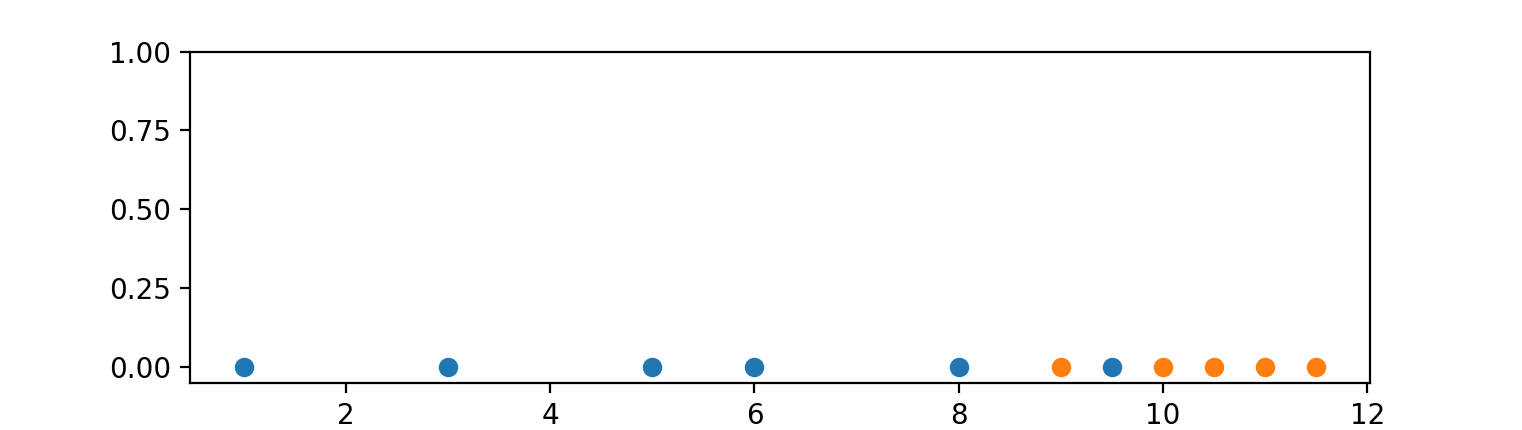
\includegraphics[width=6.2cm,height=2.5cm]{"Part 3 - Learning Systems/Unsupervised Learning/Expectation-Maximization/figures/lab_dataset.png"}
  \caption{Labeled dataset.}
  \label{fig:lab_ds}
\end{subfigure}%
\begin{subfigure}{.5\textwidth}
  \centering
  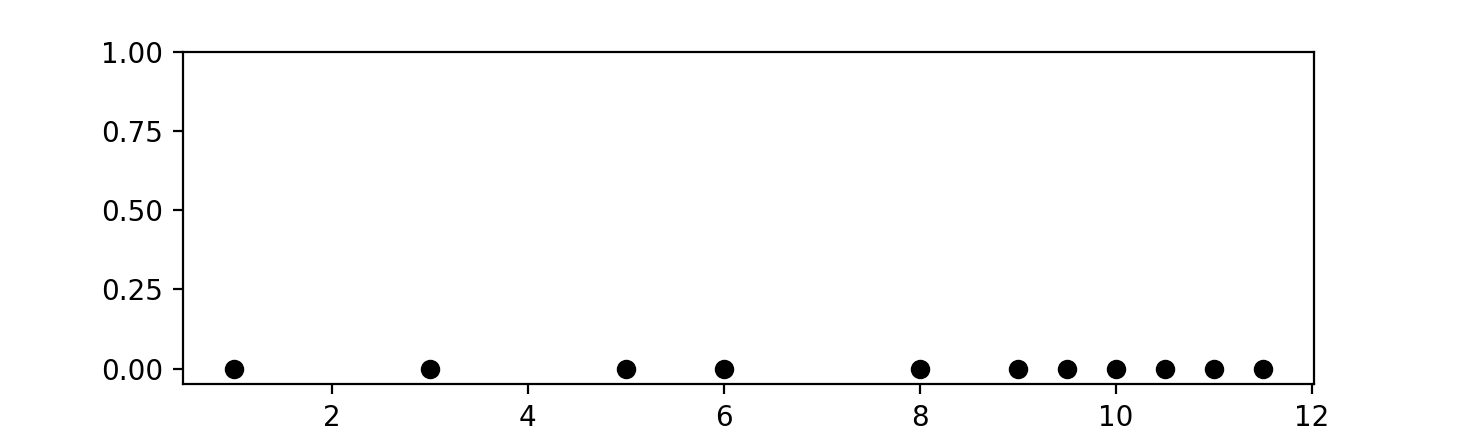
\includegraphics[width=6.2cm,height=2.5cm]{"Part 3 - Learning Systems/Unsupervised Learning/Expectation-Maximization/figures/unlab_dataset.png"}
  \caption{Unlabeled dataset}
  \label{fig:unlab_ds}
\end{subfigure}
\caption{1-dimensional dataset.}
\label{fig:ds}
\end{figure}

Taking Fig. \ref{fig:ds} (b) as example, initially the EM algorithm instantiates two Gaussian functions based on random parameters ($\mu_o$, $\sigma^{2}_o$) and ($\mu_b$, $\sigma^{2}_b$) for clusters \textit{orange} and \textit{blue}, respectively. After that, the probabilities of each example to belong to each cluster are computed. The first step is to compute the probability of each example to come from each Gaussian model (cluster) according to Equation \ref{eq:prob_clus1} (where the probability of the example $\mathbf{x}^{(i)}$ belong to the cluster $blue$ is computed):

\begin{equation}
    P(\mathbf{x}^{(i)}|b) = \frac{1}{\sqrt{2 \pi \sigma^{2}_b}} exp \left( -\frac{(\mathbf{x}^{(i)} - \mu_b)^{2}}{2\sigma^{2}_b} \right) 
    \label{eq:prob_clus1}
\end{equation}

Then, the Bayesian posterior probability of the same example being from the class $blue$ can be computed according to Equation \ref{eq:posterior}:

\begin{equation}
    b_i = P(b | x^{(i)}) = \frac{P(\mathbf{x}^{(i)}|b) P(b)}{P(\mathbf{x}^{(i)}|b) P(b) + P(\mathbf{x}^{(i)}|o) P(o)}
    \label{eq:posterior}
\end{equation}

\noindent notice that in the first step of the EM, the priors $P(b)$ and $P(o)$ are equal and both can be $0.5$, for example. For computing the posterior probability for the orange class we can use the already computed posteriors of the blue class as depicted in Equation \ref{eq:posterioro}:

\begin{equation}
    o_i = P(o | \mathbf{x}^{(i)}) = 1 - b_i
    \label{eq:posterioro}
\end{equation}

After that, the posterior probabilities for each class and examples will be computed and the Gaussian models will be shifted towards the examples that are better represented by them. For example, the blue cluster will have its parameters (mean and variance) adjusted based on the following equations, respectively:

\begin{equation}
    \mu_b = \frac{b_{1}\mathbf{x}^{(1)} + b_{2}\mathbf{x}^{(2)} + \ldots + b_{n}\mathbf{x}^{(n)}}{b_{1} + b_{2} + \ldots + b_{n}}
\end{equation}


\begin{equation}
    \sigma^{2}_b = \frac{b_{1}(\mathbf{x}^{(1)} - \mu_{b})^{2} + \ldots + b_{n}(\mathbf{x}^{(n)} - \mu_{b})^{2}}{b_{1} + b_{2} + \ldots + b_{n}}
\end{equation}

After that, the priors $P(o)$ and $P(b)$ can already be more precisely estimated and the process continues until a stop criterion is reached.

Therefore, considering the example of Figure \ref{fig:unlab_ds} where $\mathbf{X} = \{0.1, 0.3, 0.5,\\ 0.6, 0.8, 0.9, 0.95, 1.0, 1.05, 1.1, 1.15 \}$, the two Gaussian functions, blue and orange, have parameters ($\mu_{b} = 0.1$, $\sigma^{2}_{b} = 0.01$) and ($\mu_{o} = 0.3$, $\sigma^{2}_{o} = 0.01$). In order to obtain the outcomes from the pdf functions between 0 and 1, the highest \textit{peak} between both Gaussian functions was found and each $P(\mathbf{x}^{(i)}|c)$ (where $c$ stands for the class) was normalized/divided by this $peak$. The result of the first step of the EM is depicted in Figure \ref{fig:step1}. The left plot shows the initial state of the Gaussian models while the right plot shows the state of the Gaussian functions after the first M-step.

\begin{figure}[ht]
\centering
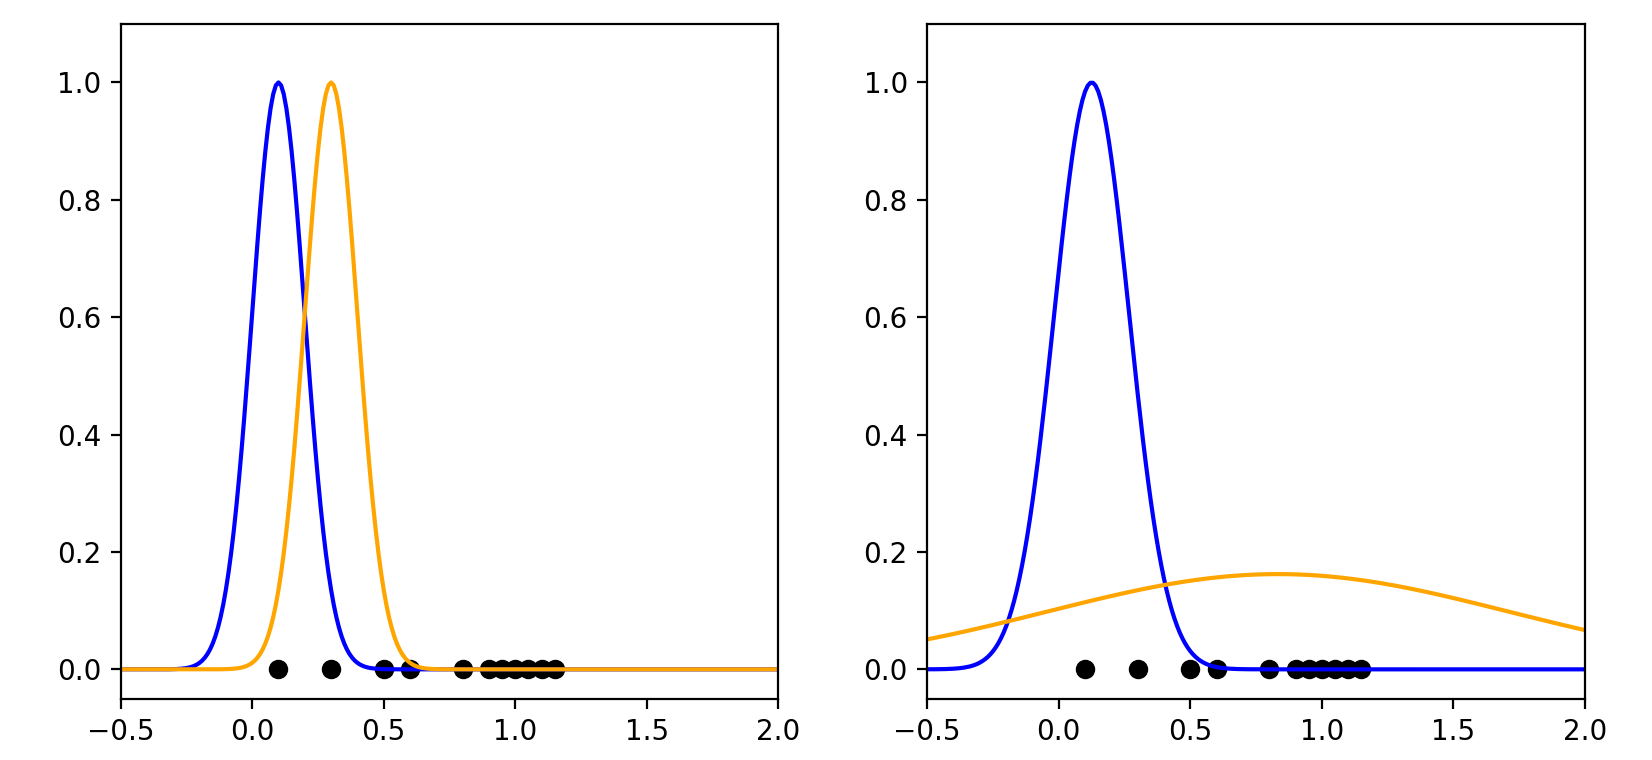
\includegraphics[width=11cm]{"Part 3 - Learning Systems/Unsupervised Learning/Expectation-Maximization/figures/step1.png"}
\caption{First step of the EM for an 1-dimensional artificial dataset.}
\label{fig:step1}
\end{figure}

%, we will obtain the vector $\mathbf{b} = \{0.99, 0.96, 0.05, 0.02e-01, 0.5e-07, 0.22e-08, 0.46e-09, 0.98e-10, 0.2e-10, 0.42e-11, 0.9e-12 \} $ and the vector $\mathbf{o} = \{0.62e-06, 0.03, 0.94, 0.99, 0.99, 0.99, 0.99, 0.99, 0.99, 0.99, 0.99\}$.

It is noticeable that the EM algorithm works similarly to the k-means algorithm, but instead of creating hard margins (i.e., no overlap among clusters) the EM creates soft margins (i.e., the probabilities of an example ($\mathbf{x}^{(i)}$) to belong to different clusters are not 0). In addition, the example exposed in this section considered a 1-dimensional dataset. For problems in the n-dimensional hyperspace (i.e., $n \geq 2$) it is necessary to use a covariance matrix instead of the simple variance. 



%\section{Mathematical foundations}
%\label{sec:math}

%Let $\mathbf{X} = \{\textbf{x}^{(1)},\ldots, \textbf{x}^{(i)},\ldots, \textbf{x}^{(N)}\}$ be a dataset containing $N$ examples such that each example $\textbf{x}^{(i)} = (x^{(i)}_1, \ldots, x^{(i)}_k, \ldots, x^{(i)}_p)$ has its corresponding target variable, $z^{(i)}$, in $\textbf{z} = \{z^{(1)}, \ldots, z^{(i)}, \ldots, z^{(N)}\}$. Be $\{\textbf{X}, \textbf{z}\}$ a sample of this data distribution so that its likelihood function takes the form $P(\textbf{X}, \textbf{z}|\theta)$, where $\theta$ represents the set of parameters of the EM model. In practice, the only knowledge about the values in $\textbf{z}$ is given by the posterior distribution $P(\textbf{z}|\textbf{X}, \theta)$. 

%The EM algorithm is aimed at maximizing the likelihood
%$P(\textbf{X}, \textbf{z}|\theta)$ by carrying out the aforementioned E-step and M-step. At this point we can use the Maximum Likelihood Estimation (MLE) method to find the statistical parameters (i.e., parameters that define a statistical distribution, for example, the mean ($\mu$) and the standard deviation ($\sigma$) of a Normal distribution) that better fit the data ($X$). The likelihood function $P(\textbf{X}, \textbf{z}|\theta)$ is differentiable and, consequently, its derivative can be used to find the parameters that maximize the 

%If the likelihood function is differentiable, the derivative test for finding maxima can be applied.

%In the E-step, we use the current parameters ($\theta^{(t)}$), to find the posterior distribution of $\textbf{z}$ given by $P(\textbf{z}|\textbf{X}, \theta)$. Then we use the posterior distribution to find the expectation of the complete data likelihood $Q(\theta, \theta^{t})$, computed as follows:

%\begin{equation}
%    Q(\theta, \theta^{t}) = \sum_{i = 1}^{N} p(z^{(i)}|\textbf{X},\theta^{t}) ln \text{ } p(\textbf{X}, z^{(i)}|\theta)
%\end{equation}

%In the M step the updated parameter $\theta^{t + 1}$ is determined by maximizing the function:

%\begin{equation}
%    \theta^{t + 1} = \underset{\theta}{\mathrm{arg max}\;} Q(\theta, \theta^{t})
%\end{equation}

%The E and M steps are alternately executed until the convergence, or a predefined stop criterion, of the algorithm is reached. Details about these steps and convergence criterion are discussed in Section \ref{sec:algorithm}. 


\section{A Gentle Introduction to Expectation Maximization}

As seen in the examples in the previous sections, the EM algorithm represents the examples from each class by using a probabilistic model for each class distribution. To represent these distributions in the same hyperspace is a problem known as \textbf{mixture models} that employs a systematic way (i.e., Maximum Likelihood Estimation - MLE) to find the parameters for each probabilistic model that better fit its respective group of examples (cluster). A mixture model can be roughly represented by the following two equations:

\begin{equation}
    p(\mathbf{x}) = \sum_{i = 1}^{k} \pi_{i} p_{i}(\mathbf{x}) 
    \label{eq:mixmodel}
\end{equation}

\begin{equation}
    \sum_{i = 1}^{k} \pi_{i} = 1
    \label{eq:mixpi}
\end{equation}

In Equations \ref{eq:mixmodel} and \ref{eq:mixpi} $k$ represents the number of statistical models in the mixture and $p(\mathbf{x})$ stands for the probabilistic function regarding any statistical distribution (e.g., Bernoulli, Gaussian (Normal), etc.) and $\pi_i$ represents the weight of the i$th$ probabilistic model.

%\section{Gaussian Mixture Models}

The Gaussian statistical models stand as the most adopted models for the EM algorithm. Therefore, Gaussian Mixture Models (GMMs) \cite{richardson1997bayesian} can be seen as a special case of the EM algorithm. %A mixture model consists in the combination of multiple probabilities distributions functions. 
The GMMs use a combination of Gaussian (or Normal $N(\mu, \Sigma)$) models such that the parameters to be optimized are the mean ($\bm{\mu}$) and covariance matrix ($\bm{\Sigma}$) from each Gaussian model. Thus, the posterior probability $p$ can be rewritten as follows: 

\begin{equation}
    p(\textbf{x} | \bm{\mu}_1, \bm{\mu}_2,\ldots, \bm{\mu}_k,\bm{\Sigma}_1, \bm{\Sigma}_2, \ldots, \bm{\Sigma}_k) = \sum_{i=1}^k \pi_{i} N(\textbf{x}| \bm{\mu}_k, \bm{\Sigma}_k).
\end{equation}

For simplicity, the set of parameters $\{ \bm{\mu}_1, \bm{\mu}_2,\ldots, \bm{\mu}_k,\bm{\Sigma}_1, \bm{\Sigma}_2, \ldots, \bm{\Sigma}_k\}$ will now be denoted by $\theta$. 

The aim of a GMM, ruled by the set of parameters $\theta$, is to precisely fit a dataset $\mathbf{X}$. For this it is necessary to estimate $\theta$ by maximizing the following likelihood function:

%Then the likelihood function is given as following:

%\begin{equation}
%    ln \text{ } p(\textbf{X}, \textbf{z}|\bm{\mu}, \bm{\sigma}^{2}) = \sum_{i=1}^n \left[ \sum_{k=1}^K \mathbf{z}^{(i)}_k N(\textbf{x}^{(i)}| \bm{\mu}_k, \bm{\sigma}_k^{2}) \right].
%\end{equation}

\begin{equation}
    log f(\mathbf{X} | \theta) = \sum_{i = 1}^{N} log \sum_{j = 1}^{k} \pi_{j} N(\mathbf{x}^{(i)} | \mu_j, \Sigma_j)
    \label{eq:mlegmm}
\end{equation}

At this point, our challenge is to optimize the parameters from Equation \ref{eq:mlegmm}. However, given the complex relationship among the parameters of the different Gaussian models it is not possible to use a mathematical framework such as gradient descent, for example. The aim of the EM algorithm is, then, to iteratively solve this problem. 

As expected, each Gaussian model must represent a subset of examples in $\mathbf{X}$. The individual influence of a particular Gaussian model (indexed by $k$) over an example $\mathbf{x}$ can be computed as follows: 

\begin{equation}
    z_k(\mathbf{x}) = \frac{\pi_k N(\mathbf{x} |\bm{\mu}_k, \bm{\Sigma}_k)}{\sum_{i=1}^K N(\mathbf{x} |\bm{\mu}_i, \bm{\Sigma}_i)}.
\end{equation}

So, $z_k(\mathbf{x})$ can be seen as the probability of the example $\mathbf{x}$ being represented by the k$th$ Gaussian model. As aforementioned, there is not a formal method for estimating the set of parameters $\theta$, however, these parameters can be updated as follows: 

\begin{equation}
    \bm{\mu}_k^{new} = \frac{1}{N_k} \sum_{i=1}^{N_k} z_k(\mathbf{x}^{(i)}) \mathbf{x}^{(i)}
\label{mu_new}
\end{equation}

\begin{equation}
    \bm{\Sigma}_k^{new} = \frac{1}{N_k} \sum_{i=1}^{N_{k}} z_k(\mathbf{x}^{(i)}) (\mathbf{x}^{(i)} - \bm{\mu}_k^{new}) (\mathbf{x}^{(i)} - \bm{\mu}_k^{new})^{T}
\label{sigma_new}
\end{equation}

\begin{equation}
    \pi_k^{new} = \frac{N_k}{N}
    \label{pi_new}
\end{equation}

\noindent In Equations \ref{mu_new}, \ref{sigma_new} and \ref{pi_new}, $N_k = \sum_{i = 1}^{N} z_k(\mathbf{x}^{(i)})$. In addition, they are not supposed to directly maximize Equation \ref{eq:mlegmm}. In fact, they seek for the optimal parameters of the following similar Equation:

\begin{equation}
     \hat{f}(\mathbf{X} | \theta) = \sum_{i = 1}^{N} \sum_{j = 1}^{k} z_{j}(\mathbf{x^{(i)}}) log \frac{\pi_{j} N(\mathbf{x}^{(i)} | \mu_j, \Sigma_j)}{z_{j}(\mathbf{x^{(i)}})}
\end{equation}


%Adicionalmente, as equações (12–14) não buscam maximizar precisamente o logaritmo da verossimilhança sobre θ, dado pela equação (6). Na verdade, essas equações buscam maximizar uma função auxiliar do logaritmo da verossimilhança, a esperança do logaritmo da verossimilhança, que é derivado da equação (6), usando a desigualdade de Jensen. Essa função auxiliar é dada por:

%The value of $\mathbf{z}_{k}^{(i)}$ respects the constraint: $\sum_{k=1}^K \mathbf{z}^{(i)}_k=1$. This can be interpreted as the influence (weight) of each distribution takes on to example $\textbf{x}_i$. After some algebra, the value of $\mathbf{z}^{(i)}_k$ that satisfies the restriction is computed in the E step of GMM algorithm as following:

%\begin{equation}
%    z_{ik}^{new} = \frac{N(x_i|\bm{\mu}_k^{new}, \bm{\sigma}_k^{2})}{\sum_{k=1}^K N(x_i|\bm{\mu}_j^{new}, \bm{\sigma}_j^{2})}.
%\label{z_new}
%\end{equation}

%In the M step, the parameters $\bm{\mu}$ and $\bm{\sigma}$ of the Normal pdf are computed as follows:

%\begin{equation}
%    \bm{\mu}_k^{new} = \frac{1}{N_k} \sum_{i=1}^N z^{(i)}_k^{new} \textbf{x}^{(i)},
%\label{mu_new}
%\end{equation}

%\begin{equation}
%    \bm{\sigma}_k^{new}^{2} = \frac{1}{N_k} \sum_{i=1}^N z^{(i)}_k^{new} (\textbf{x}^{(i)}-\bm{\mu}_k^{old})(\textbf{x}^{(i)}-\bm{\mu}_k^{old})^T,
%\label{sigma_new}
%\end{equation}

%\noindent where $N_k$ is given as:

%\begin{equation}
%    N_k = \sum_{i=1}^N z^{(i)}_k^{new}.
%\end{equation}

%After the convergence of the GMM algorithm, i.e., when the parameters don't change anymore, the estimated $\textbf{x}^{(i)}^{new}$ is computed as:

%\begin{equation}
%    \textbf{x}^{(i)}^{new} = \sum_{i=1}^N z^{(i)}_k^{new} \bm{\mu}_k^{new}
%\end{equation}

Figure \ref{example_mixture} shows an example of a Gaussian Mixture Model (GMM) using three Gaussian models. The mean parameter of the Gaussian models are, respectively, $5$, $10$ and $17$; they share the same variance, i.e., 2. Dotted lines indicate the Gaussian models and the continuous line shows the resulting GMM. Each Gaussian model has $\pi_k = \frac{1}{3}$. 

\begin{figure}[ht]
\centering
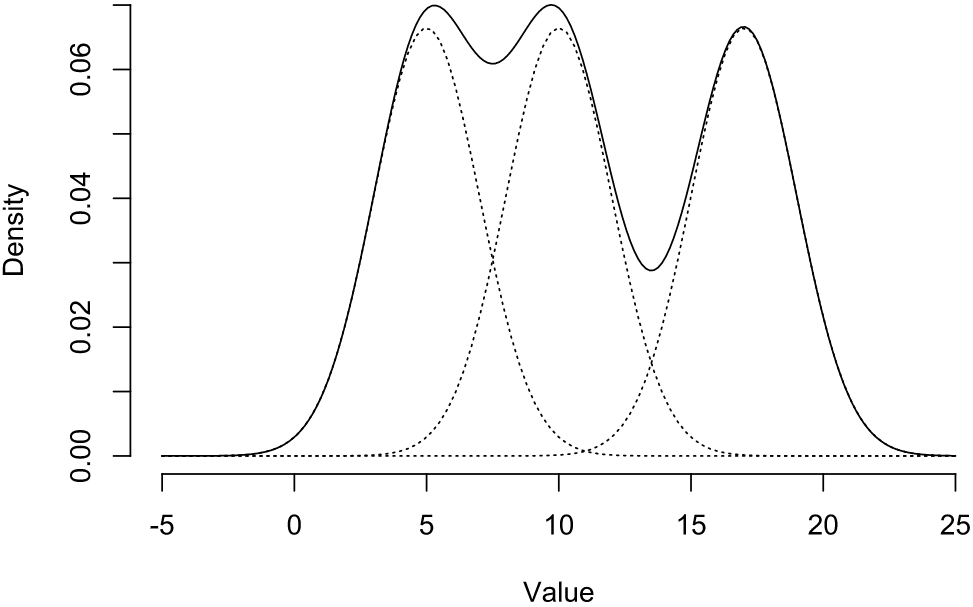
\includegraphics[width=11cm]{"Part 3 - Learning Systems/Unsupervised Learning/Expectation-Maximization/figures/gaussian_mixture.png"}
\caption{Example of Gaussian mixture. Adapted from \cite{Smason79}.}
\label{example_mixture}
\end{figure}

\subsection{The role of the Covariance Matrix ($\Sigma$)}

The covariance matrix $\bm{\Sigma}$ provides the algorithm with the ability to identify clusters of different shapes and sizes. The diagonal values of the matrix contains the variances of the respective features of the problem: the bigger these values, the more spread out the cluster is. Values that outsize the matrix diagonal quantifies the covariance between pairs of problem features. From covariance values the correlation between problem features can be computed.

In order to illustrate the importance of covariance matrix $\bm{\Sigma}$, Figure \ref{example_partition} shows an example of a simple data set and resulting partitions after applying the well known K-Means algorithm and the EM algorithm for the spacial case when $\bm{\Sigma}$ is a diagonal matrix. 

\begin{figure}[ht]
\centering
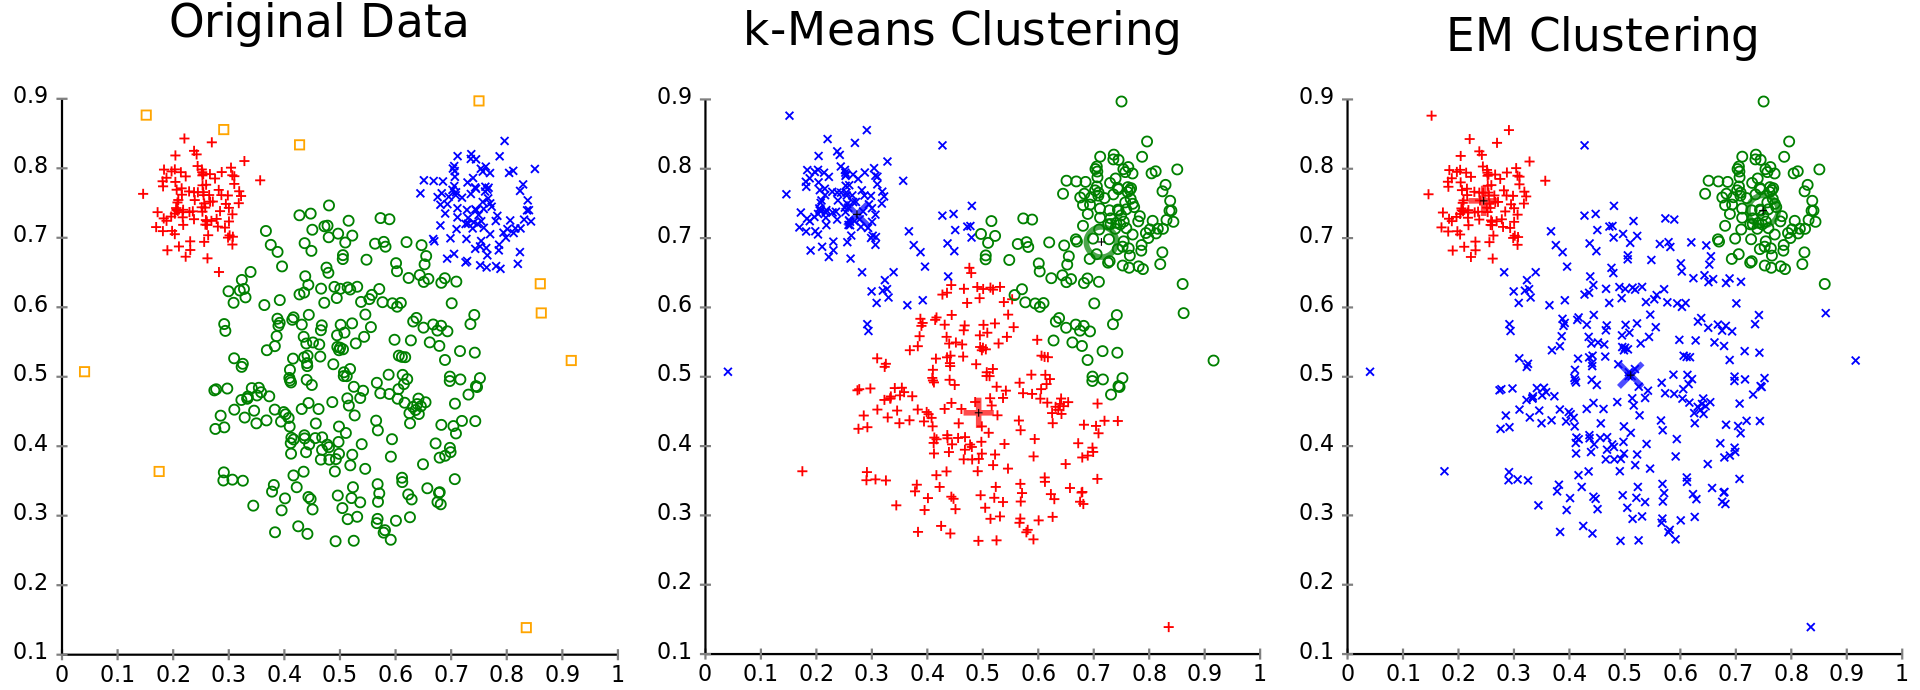
\includegraphics[width=13cm]{"Part 3 - Learning Systems/Unsupervised Learning/Expectation-Maximization/figures/ClusterAnalysis_Mouse.png"}
\caption{Example of partitions found by K-Means and EM clustering algorithms. Adapted from \cite{Chire}.}
\label{example_partition}
\end{figure}

The original data set contains three classes with different spherical sizes. After applying K-Means clustering algorithm, the resulting partition is different from original one since this algorithm divides the space into clusters of equal dispersion. In other words, K-Means finds spherical clusters of equal sizes. On the other hand, after applying EM algorithm, the resulting partition is similar to original one. This is because EM algorithm is able to create a model that identifies different distributions, which allows to find a resulting partition with clusters of different sizes and shapes.

\section{The EM Algorithm}
\label{sec:algorithm}

%EM is broadly used in Machine Leaning applications because EM algorithm is simple and easy to understand. Algorithm \ref{pseudocod} shows the main steps.

The EM algorithm can be characterized by two main steps: Expectation (E-step) and Maximization (M-step). In the E-step, the algorithm computes the expected value of a dataset example using the current estimate of the parameter. In the M-step, the algorithm uses information from previous step to define a maximum-likelihood estimate of the parameters. Figure \ref{EM-algorithm} shows an overall flow chart for the EM algorithm.


\begin{figure}[ht]
\centering
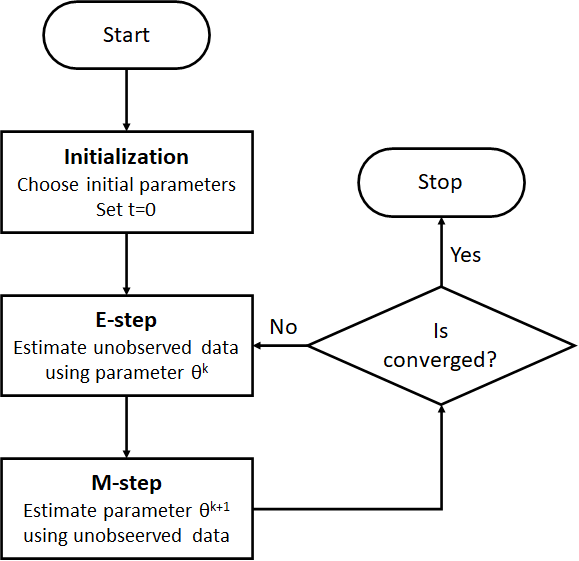
\includegraphics[width=9cm]{"Part 3 - Learning Systems/Unsupervised Learning/Expectation-Maximization/figures/algorithm.png"}
\caption{Flow chart for EM algorithm.}
\label{EM-algorithm}
\end{figure}


Algorithm \ref{pseudocod} presents the pseudo-code for the EM method. The E-step and M-step are executed until one or more convergence criterion are satisfied. Examples of convergence criteria are presented in Algorithm \ref{pseudocod}.

%%%%%%%%%%%%%%%%%%%%%%%% ALGORITHM
\begin{algorithm}[ht]
	%\renewcommand{\baselinestretch}{0.8}
	\caption{EM algorithm}
	\label{pseudocod}
    
    Parameters: Dataset $\textbf{X}$, number of clusters $k$.
    
    Output: Final partition.
    
	\begin{algorithmic}[1] 
		\STATE{Choose initial parameters. Set time $t=0$. Set $\epsilon$.}
		
        \REPEAT
		
		\STATE \textbf{E-step}: find the values $\pi_{k}$ (for $k = {1,2,\ldots,k}$) using the Equation \ref{pi_new}
		
		\STATE \textbf{M-step}: update the parameters $\bm{\mu}_k$ and $\bm{\Sigma}_k$ (for $k = {1,2,\ldots,k}$) using equations \ref{mu_new} and \ref{sigma_new}, respectively
				
		\UNTIL one of the following criteria is satisfied:
   \begin{itemize}
       \item the maximum number of iterations is reached;
       \item there is no more difference between the current and previous partitions; or
       \item the difference between the likelihood function values at iteration $t$ and $t-1$ is smaller than a predefined threshold $\epsilon$.
   \end{itemize}  
	\end{algorithmic}
	
\end{algorithm}
%%%%%%%%%%%%%%%%%%%%%%%% ALGORITHM



\section{Applications}
\label{sec:applications}

Due to the importance of the EM algorithm for the Machine Learning field, several researchers have applied it to a wide variety of real problems. These problems are concerned about Natural Language Processing, Signal Processing, medical image reconstruction and so on. This section briefly present some studies that applied EM algorithm as tool for solving real problems.

Ramme et al. (2009) \cite{ramme2009semi} used the EM algorithm to segment the hand phalanx bones. The goal of this work is to  analyze whether a semi-automated technique will improve the efficiency while providing similar definitions as compared to a human rater. %Figure \ref{EM-bone} shows surface models of the anterior aspects of the 12 phalanx bones after using EM algorithm.

%\begin{figure}[ht]
%\centering
%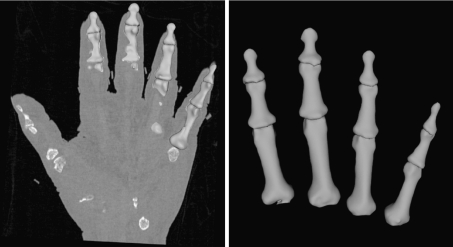
\includegraphics[width=8cm]{figures/EM_bone.png}
%\caption{Computed Tomography image of the hand (left) and the posterior aspects of the bone models pictured alone (right) (from \cite{ramme2009semi}).}
%\label{EM-bone}
%\end{figure}

Kujawinska et al. (2016) \cite{kujawinska2016} applied the EM algorithm to support purchasing decisions in the welding industry. Authors analyzed the EM for the selection of material (212 combinations of flux and wire melt) for the SAW (Submerged Arc Welding) method process. The work showed that each of the
212 records can be assigned with a probability of affiliation to all the four clusters used in the experiments. These probabilities allow the user to make a better decision, since cases with ambiguous assignment can be better analyzed.

Subudhi et al. (2020) \cite{subudhi2020automated} used the Expectation Maximization method and the Random Forest classifier for automated segmentation and classification of brain stroke. The part of the brain affected by the stroke was segmented using the EM algorithm and Magnetic Resonance Imaging (MRI) of brains. %Figure \ref{EM-MRI} shows the application of EM algorithm in the process of brain lesion detection.

%\begin{figure}[ht]
%\centering
%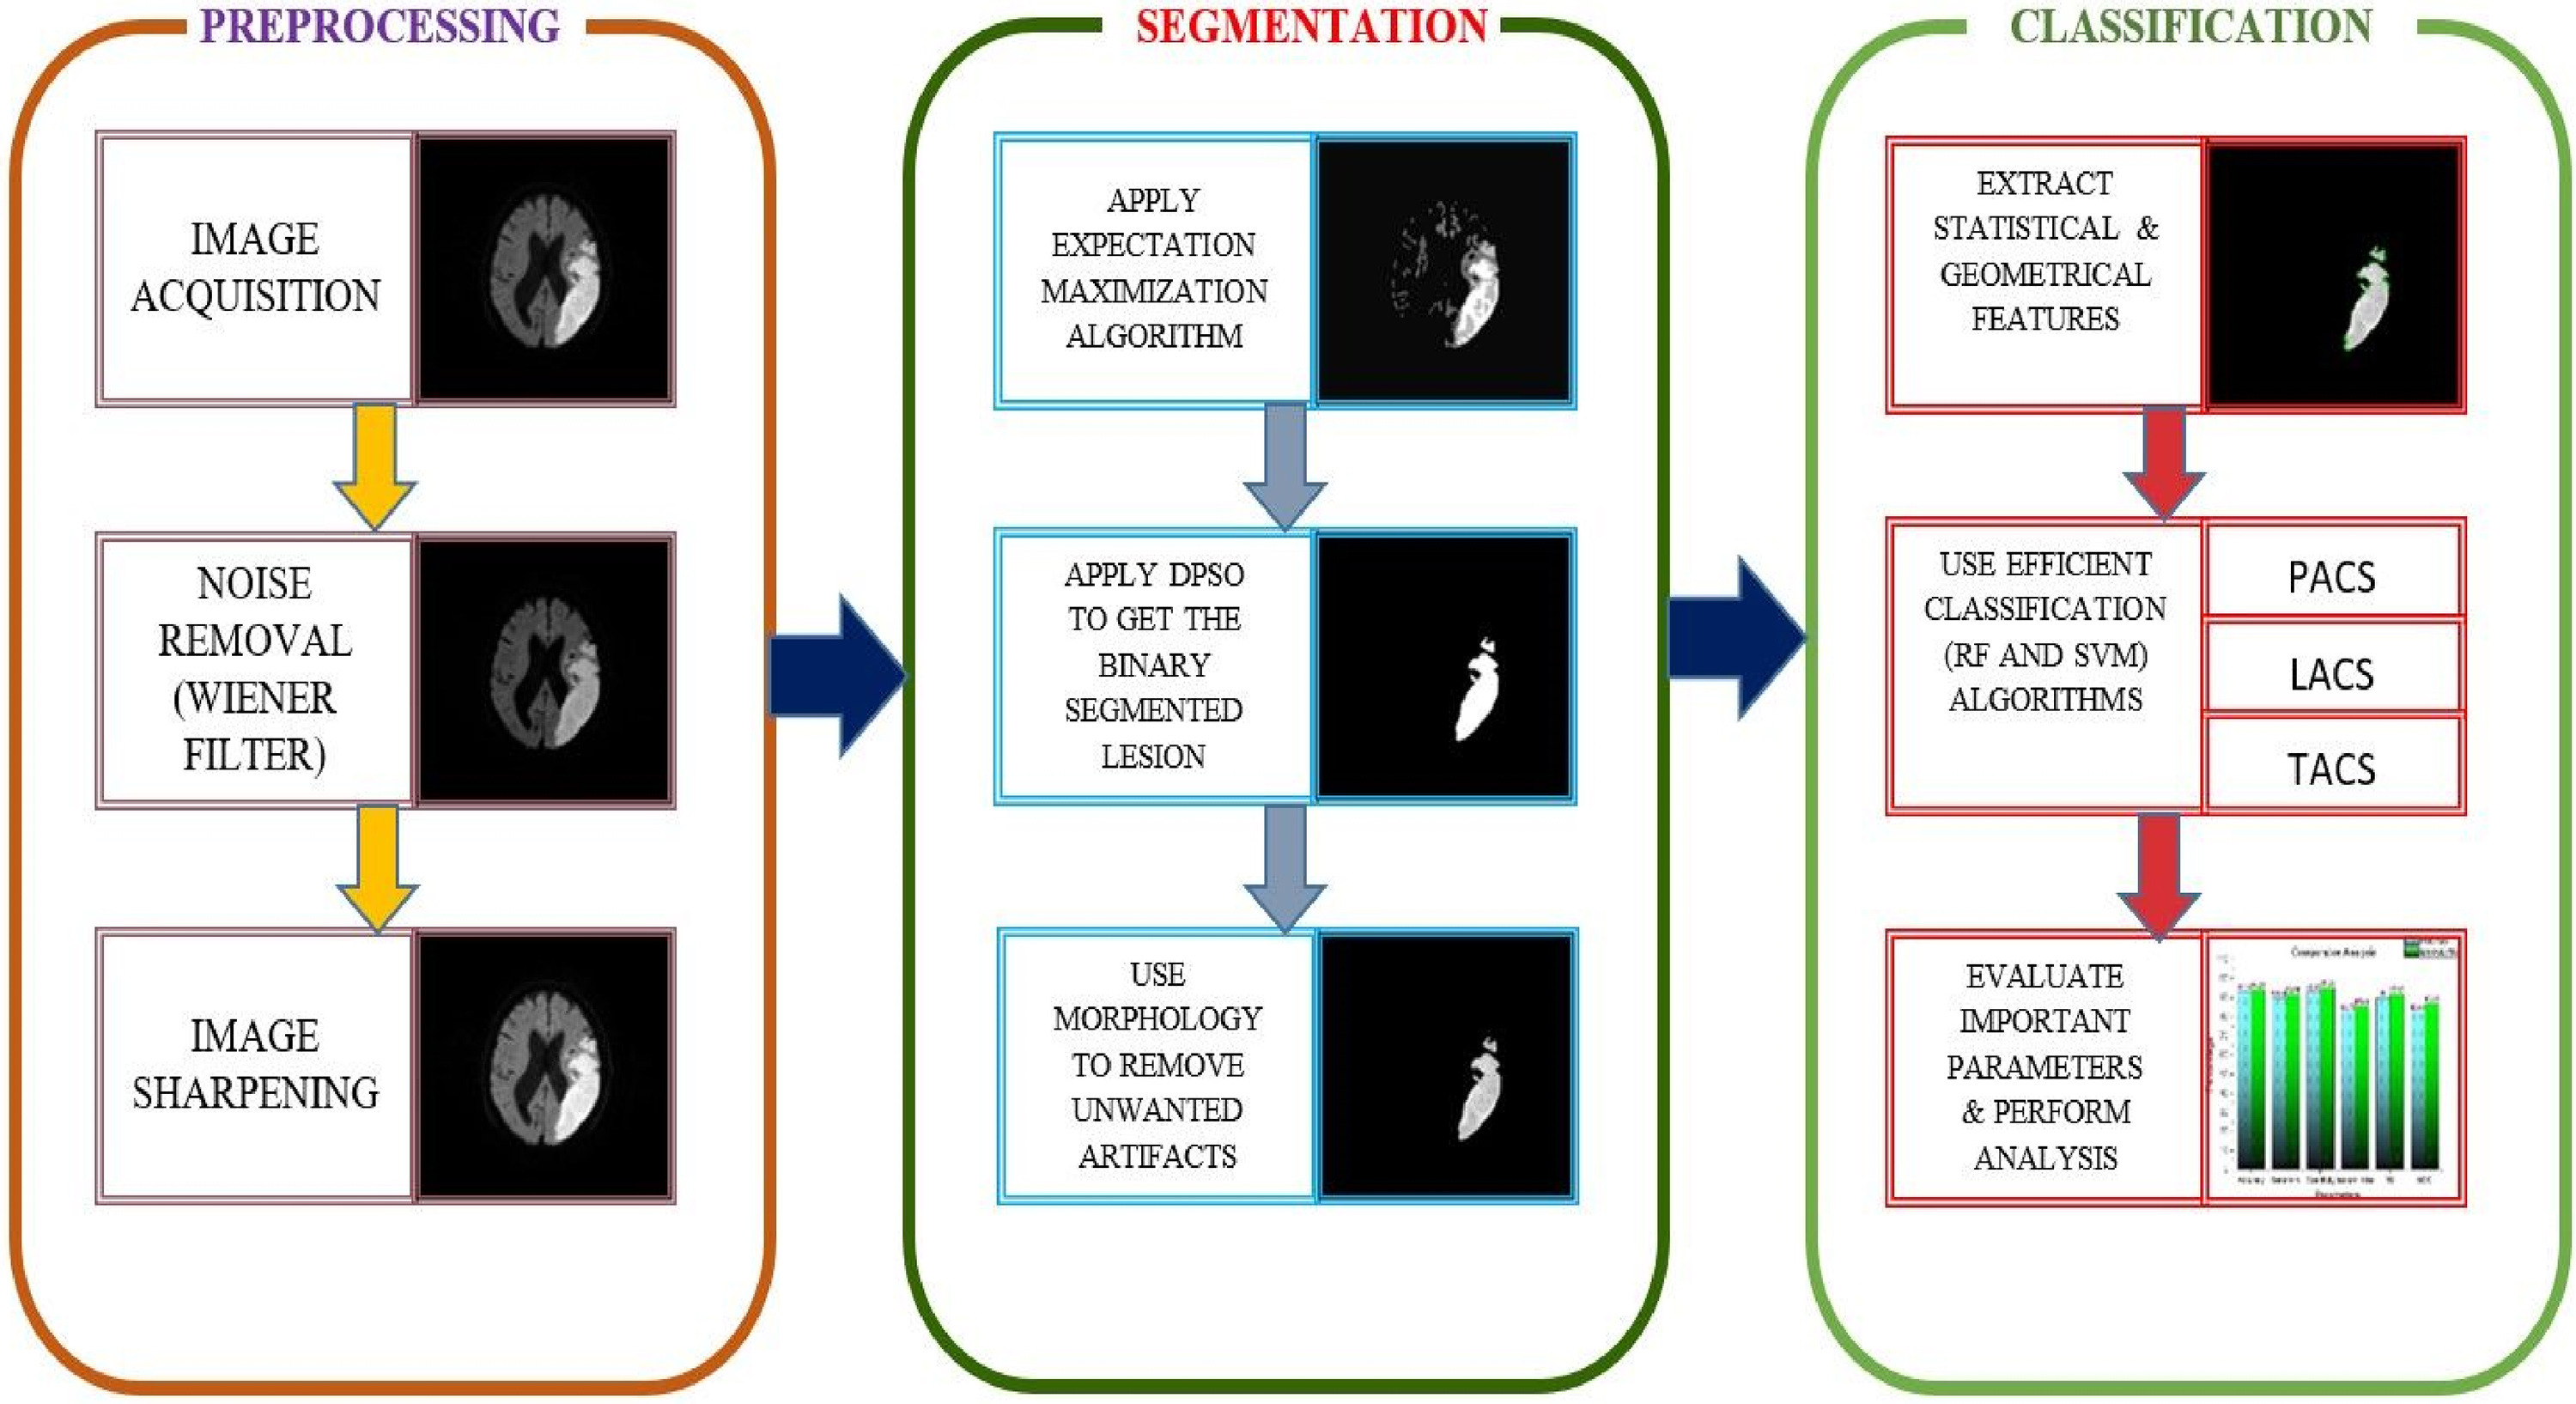
\includegraphics[width=10cm]{figures/EM-MRI.png}
%\caption{Illustration of EM based method for lesion detection using MRI image (from %\cite{subudhi2020automated}).}
%\label{EM-MRI}
%\end{figure}

Lakshminarayanan et al. (2020) \cite{lakshminarayanan2020new} recovered the high-resolution image of a corresponding low-resolution image. For this, the authors proposed a new integrated approach based on the iterative super-resolution algorithm and the EM method for face hallucination (the process of improving a low resolution -- LR -- image to a high resolution -- HR -- image without altering the originality of the image). %Figure \ref{EM-image} shows the global face model learning.

%\begin{figure}[ht]
%\centering
%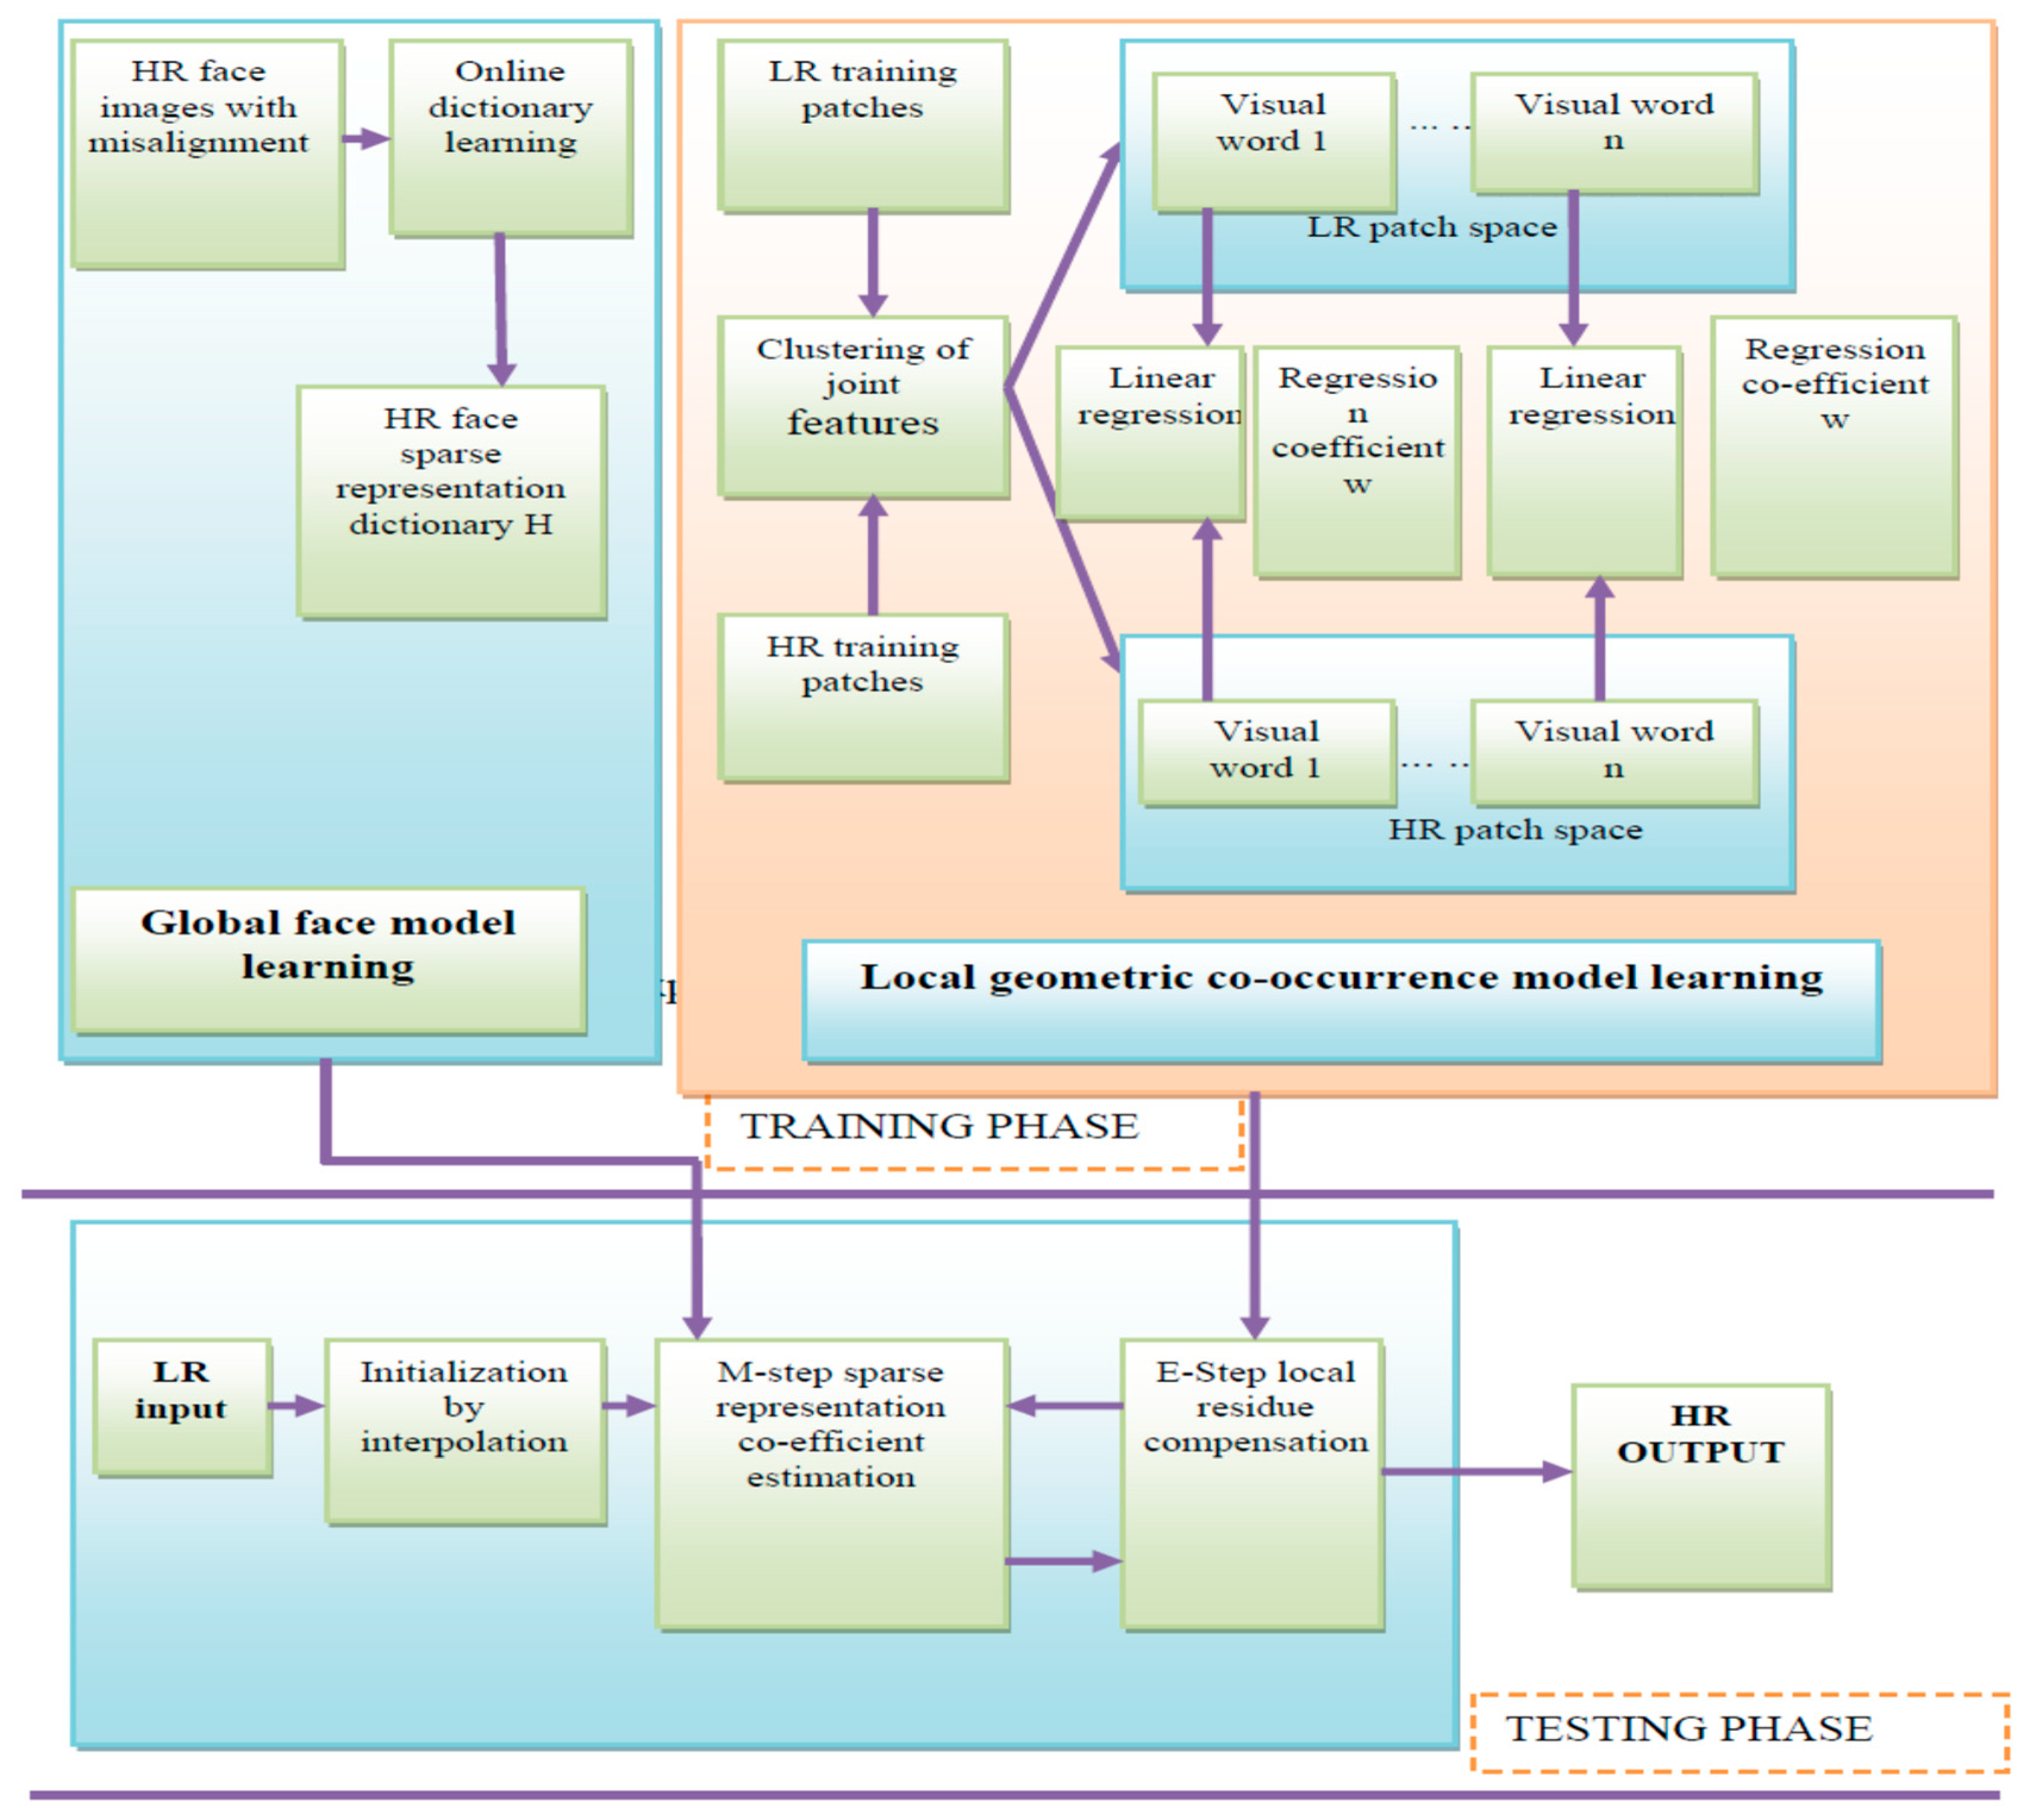
\includegraphics[width=10cm]{figures/EM-image.png}
%\caption{Overview of model learning for the proposed approach (from %\cite{lakshminarayanan2020new}).}
%\label{EM-image}
%\end{figure}

\section{Exercises}

\begin{enumerate}
    \item Based on the experiment presented in Section \ref{sec:coin}, use EM algorithm to estimate the bias of each coin after 100 iterations.
    \item Use 300 samples of Gaussian Mixture with mixing probability equal to 1/3 as follow:
    \begin{equation*}
        X_1 \sim N\left( \begin{bmatrix} 1 \\ 1 \end{bmatrix}, \begin{bmatrix} 1 & 4 \\ 4 & 1 \end{bmatrix} \right)
    \end{equation*}
    
    \begin{equation*}
        X_2 \sim N\left( \begin{bmatrix} 5 \\ 5 \end{bmatrix}, \begin{bmatrix} 4 & 2 \\ 2 & 6 \end{bmatrix} \right)
    \end{equation*}
    
    \noindent and implements the EM algorithm to estimate its parameters.
    
    \item Show a scatter plot of the above dataset for different values of mixing probability: 1/2, 1/3, 1/4 and 1/5. What can you observe from the results?
    
    \item Changing the dataset to:
    
    \begin{equation*}
        X_1 \sim N\left( \begin{bmatrix} 1 \\ 1 \end{bmatrix}, \begin{bmatrix} 1 & 4 \\ 4 & 1 \end{bmatrix} \right)
    \end{equation*}
    
    \begin{equation*}
        X_2 \sim N\left( \begin{bmatrix} 5 \\ 5 \end{bmatrix}, \begin{bmatrix} 4 & 2 \\ 2 & 6 \end{bmatrix} \right)
    \end{equation*}
    
    \begin{equation*}
        X_3 \sim N\left( \begin{bmatrix} 3 \\ 3 \end{bmatrix}, \begin{bmatrix} 1 & 1 \\ 1 & 1 \end{bmatrix} \right)
    \end{equation*}
    
    \noindent repeat the question 3. What can you observe from the new results?
    
\end{enumerate}

    

\bibliographystyle{unsrt}
\bibliography{bibliography}

